\chapter{Prototype haute performance}
\label{chap:protoHP}

Dans le cadre d'application qu'est la réalité augmentée spatiale, les interactions jouent un rôle majeur dans l'expérience de l'utilisateur. Ainsi, la réactivité, la fluidité de l'expérience et la latence générale du système sont des points cruciaux qu'il est impossible de négliger. Pour pouvoir atteindre ces objectifs et pouvoir pousser les applications encore plus loin, aussi bien dans l'interaction que dans le rendu ou dans le contenu, sans avoir besoin d'une puissance de calcul dépassant l'entendement, une optimisation à la fois logicielle, matérielle et architecturale est nécessaire. 
Cette optimisation a fait l'objet d'une grande partie de mon stage et m'a amené à développer un prototype dit "haute performance" des outils que propose \texttt{RealityTech}. L'optimisation logicielle s'est portée sur l'amélioration des performances des algorithmes de traitement d'image, bien connus pour être extrêmement consommateurs des ressources. Pour l'optimisation matérielle, la tâche fut quelque peu différente. En effet, nous nous sommes attelés à effectuer des mesures et des calculs sur la puissance théorique du matériel, la latence réelle des caméra ainsi que la rapidité de l'encodage des flux vidéos, pour arriver à établir les performances réelles qu'il nous était possible d'atteindre avec différentes combinaisons de matériel. Enfin, le développement du prototype s'est achevé avec la création d'une nouvelle architecture logiciel en micro services\cite{dmitry2014micro}. Le but était de créer un environnement modulaire réactif, où les services peuvent mourir sans pour autant mettre en péril tout le système et ainsi améliorer grandement la qualité générale des outils fournis.

\section{Amélioration logicielle}
\label{sec:hpsoft}
De nos jours, les optimisations font l'objet de développements ciblés et très spécifiques, se concentrant la plupart du temps sur l'amélioration d'un unique point crucial d'un algorithme ou d'une application. Dans notre cas, l'optimisation logicielle a surtout été effectuée au niveau des algorithmes de traitement d'image, omniprésents et indispensables à la technologie. La réalité augmentée spatiale a besoin du monde réel pour exister, c'est pourquoi le matériel se compose de nombreux capteurs (caméras) pour l'analyser et que de nombreux algorithmes de traitement des données captées (images) sont mis en place. 
Après une rapide analyse du logiciel existant, il est indéniable que le traitement le plus utilisé est la convolution d'une image par un filtre qui possède un nombre incalculable d'applications. C'est pourquoi nous avons choisit de concentrer nos efforts sur l'optimisation de ce dernier.

\subsection{Convolution - Théorie}
\begin{quotation}
\textit{En mathématiques, le produit de convolution est un opérateur bilinéaire et un produit commutatif, généralement noté $∗$, qui, à deux fonctions f et g sur un même domaine infini, fait correspondre une autre fonction $f * g$ sur ce domaine, qui en tout point de celui-ci est égale à l'intégrale sur l'entièreté du domaine (ou la somme si celui-ci est discret) d'une des deux fonctions autour de ce point, pondérée par l'autre fonction autour de l'origine — les deux fonctions étant parcourues en sens contraire l'une de l'autre (nécessaire pour garantir la commutativité).\footnote{Source: \href{https://fr.wikipedia.org/wiki/Produit_de_convolution}{Produit de convolution - Wikipedia}}}
\end{quotation}

Dans le cadre du traitement d'image, le produit de convolution représente une technique de filtrage d'image visant à accentuer ou atténuer certaines caractéristiques de celle-ci telles que la netteté, le flou ou les zones de fort gradient (les contours) par exemple (Figure~\ref{fig:conv:filter}). Étant donné que nous travaillons avec des images définies par un nombre fini de pixels, la convolution d'une image est réalisée dans le domaine discret où $f$ et $g$, dans la définition mathématique, représentent respectivement une image et le filtre qu'on souhaite lui appliquer. Le résultat de cette convolution est une nouvelle image.

On appelle filtre, ou noyau de convolution, une image (ou une matrice), généralement de petite taille, définie en amont, qui va être utilisée pour calculer la nouvelle valeur de chacun des pixels de l'image résultat. C'est la définition de ce dernier qui va décider du traitement appliqué à l'image. 

Le calcul de la valeur d'un pixel dans l'image résultat se fait de la manière suivante : Le voisinage autour du pixel dont on souhaite calculer la valeur est, pondéré par le filtre de convolution que l'on aura préalablement centré sur ce pixel. La nouvelle valeur du pixel représente la somme de toutes les valeurs précédemment calculées (Algorithme~\ref{algo:pseudo:cpu:conv}). Prenons un exemple concret. Sur la Figure~\ref{fig:conv:image}, on souhaite calculer la nouvelle valeur du pixel positionné en 3,3 dans l'image d'origine (I). On sélectionne donc un voisinage de même taille que le filtre (K) centré sur ce pixel, dont chaque élément va être multiplié par la valeur du filtre afin de calculer la valeur du pixel 3,3 dans la nouvelle image soit: 
\begin{center}
$I_{3,3} * K = 88 * 1/9 + 21 * 1/9 + 25 * 1/2 + 68 * 1/9 + 14 * 1/9 + 15 * 1/9 + 35 * 1/9 + 52 * 1/9 + 10 * 1/9 = 36$
\end{center}.

\begin{figure}[H]
\centering
	\subfloat[Image originale]{
      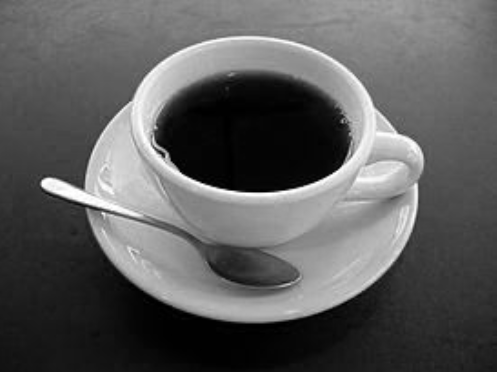
\includegraphics[width=0.33\textwidth]{images/coffee-identity}
      \label{sub:conv:filter:original}
      }
     \subfloat[Filtre contour]{
      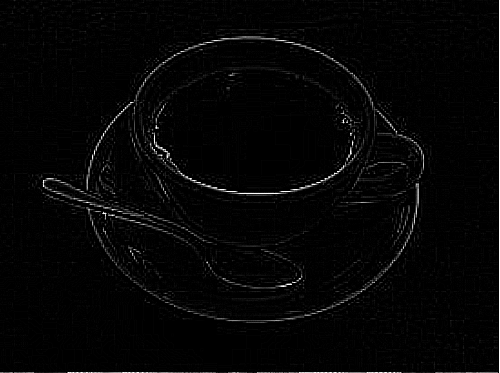
\includegraphics[width=0.33\textwidth]{images/coffee-outline}
      \label{sub:conv:filter:outline}
      }
      \\
      	\subfloat[Filtre de netteté]{
      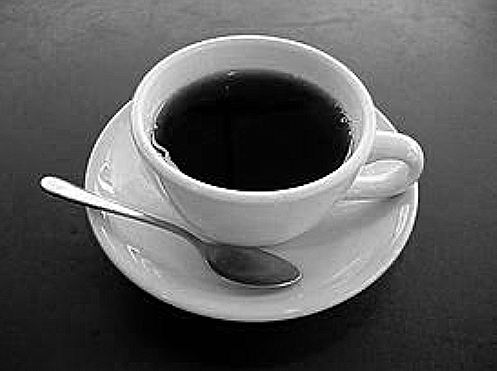
\includegraphics[width=0.33\textwidth]{images/coffee-sharpen}
      \label{sub:conv:filter:sharpen}
      }
     \subfloat[Filtre relief]{
      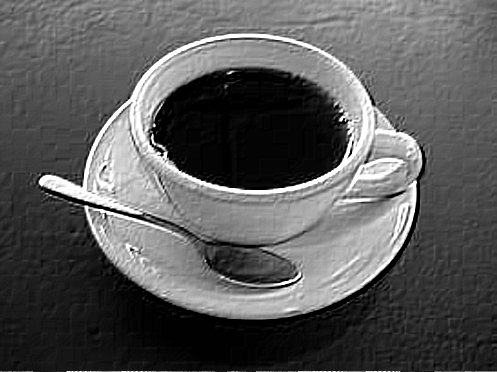
\includegraphics[width=0.33\textwidth]{images/coffee-emboss}
      \label{sub:conv:filter:emboss}
      }
\caption{Différents filtres de convolution appliqués à une image.}
\label{fig:conv:filter}
\end{figure}

\begin{figure}[H]
\centering
\begin{tikzpicture}
	\matrix (mtr) [matrix of nodes,row sep=-\pgflinewidth, nodes={draw,  minimum size=5.7mm, anchor=center}]
	{
		12 & 46  & 05 & 94 & 25 & 00 & 87\\
		05 & 13  & 01 & 20 & 25 & 00 & 37\\
		72 & 25  & |[fill=red!30]| 88 & |[fill=red!30]| 21 & |[fill=red!30]| 25 & 00 & 99\\
		21 & 74  & |[fill=red!30]| 68 & |[fill=red!30]| 14 & |[fill=red!30]| 15 & 00 & 61\\
		48 & 97  & |[fill=red!30]| 35 & |[fill=red!30]| 52 & |[fill=red!30]| 10 & 00 & 42\\
		11 & 29  & 57 & 00 & 75 & 00 & 12\\
		17 & 01  & 78 & 00 & 50 & 00 & 12\\
		16 & 54  & 00 & 00 & 25 & 00 & 11\\
	};

	\draw[very thick, red] (mtr-3-3.north west) rectangle (mtr-5-5.south east);

	\node [below= of mtr-8-4.south] (lm) {$\bf I$};
	\node[right = 0.2em of mtr] (str) {$* \frac{1}{9}$};

	\matrix (K) [right=0.2em of str,matrix of nodes,row sep=-\pgflinewidth, nodes={draw, fill=blue!30,  minimum size=5.7mm, anchor=center}]
	{
		1 & 1 & 1 \\
		1 & 1 & 1 \\
		1 & 1 & 1 \\
	};
	\node [below = of K-3-2.south] (lk) {$\bf K$};

	\node [right = 0.2em of K] (eq) {$=$};

	\matrix (ret) [right=0.2em of eq,matrix of nodes,row sep=-\pgflinewidth, nodes={draw, minimum size=5.7mm, anchor=center}, nodes in empty cells]
	{
		 &   &  &  &  &  & \\
		 &   &  &  &  &  & \\
		 &   &  &  &  &  & \\
		 &   &  & |[fill=green!30]| 36 &  &  & \\
		 &   &  &  &  &  & \\
		 &   &  &  &  &  & \\
		 &   &  &  &  &  & \\
		 &   &  &  &  &  & \\
	};
	\node [below = of ret-8-4.south] (lim) {${\bf I_{i,j}} * {\bf K}$};

	\draw[very thick, green] (ret-4-4.north west) rectangle (ret-4-4.south east);

	\draw[densely dotted, blue, thick] (mtr-3-3.north west) -- (K-1-1.north west);
	\draw[densely dotted, blue, thick] (mtr-5-3.south west) -- (K-3-1.south west);
	\draw[densely dotted, blue, thick] (mtr-3-5.north east) -- (K-1-3.north east);
	\draw[densely dotted, blue, thick] (mtr-5-5.south east) -- (K-3-3.south east);

	\draw[densely dotted, green, thick] (ret-4-4.north west) -- (K-1-1.north west);
	\draw[densely dotted, green, thick] (ret-4-4.south west) -- (K-3-1.south west);
	\draw[densely dotted, green, thick] (ret-4-4.north east) -- (K-1-3.north east);
	\draw[densely dotted, green, thick] (ret-4-4.south east) -- (K-3-3.south east);

	\draw[very thick, blue] (K-1-1.north west) rectangle (K-3-3.south east);

	\node[anchor=south east, inner sep=0.01em, blue] at (mtr-3-3.south east) (xx) {\scalebox{.5}{$\times 1$}};
	\node[anchor=south east, inner sep=0.01em, blue] at (mtr-3-4.south east) (xx) {\scalebox{.5}{$\times 1$}};
	\node[anchor=south east, inner sep=0.01em, blue] at (mtr-3-5.south east) (xx) {\scalebox{.5}{$\times 1$}};
	\node[anchor=south east, inner sep=0.01em, blue] at (mtr-4-3.south east) (xx) {\scalebox{.5}{$\times 1$}};
	\node[anchor=south east, inner sep=0.01em, blue] at (mtr-4-4.south east) (xx) {\scalebox{.5}{$\times 1$}};
	\node[anchor=south east, inner sep=0.01em, blue] at (mtr-4-5.south east) (xx) {\scalebox{.5}{$\times 1$}};
	\node[anchor=south east, inner sep=0.01em, blue] at (mtr-5-3.south east) (xx) {\scalebox{.5}{$\times 1$}};
	\node[anchor=south east, inner sep=0.01em, blue] at (mtr-5-4.south east) (xx) {\scalebox{.5}{$\times 1$}};
	\node[anchor=south east, inner sep=0.01em, blue] at (mtr-5-5.south east) (xx) {\scalebox{.5}{$\times 1$}};
\end{tikzpicture}
\caption{Convolution d'une matrice (image) (I) par un filtre (K)}
\label{fig:conv:image}
\end{figure}

\begin{algorithm}[H]
	\caption{Convolution d'une image par un filtre}
	\begin{algorithmic}
		\Procedure{Convolution}{I, K, Iw, Ih, Ks}\Comment{I: image, K: filtre}
		\State $I_{conv} \gets I$
		\State $Khs \gets floor(Ks \div 2)$
		\State $x \gets 0, y \gets 0$
		\State $sum \gets 0$
		\For{$x \leq Iw ; ++x$}
			\For{$y \leq Ih ; ++y$}\Comment{Pour tous les pixels $x,y$}
				\For{$i \leq Ks ; ++j$}
					\For{$j \leq Ks ; ++j$}\Comment{Pour chaque élément dans une fenêtre de taille $Ks$}
					\State ${pos_x \gets x + i - Ksh}$ \Comment{pos = pos + position dans le voisinage}
					\State ${pos_y \gets y + j - Ksh}$ \Comment{pos = pos + position dans le voisinage}
					\If{$outOf(I, pos_x, pos_y)$} \Comment{Vérifie que les positions sont dans l'image (bords)}
						\State $continue$
					\EndIf
					\State $sum \gets sum + I_{pos_x, pos_y} * K{i, j}$ \Comment{Somme du voisinage par le filtre}
					\State $maskSum \gets maskSum + K{i, j}$
					\EndFor
				\EndFor
				\State $I_{conv}{x, y} \gets sum \div maskSum$ \Comment{Valeur finale = somme normalisée}
			\EndFor
		\EndFor
		\State \Return $I_{conv}$ \Comment{Retourne la nouvelle image}
		\EndProcedure
	\end{algorithmic}
	\label{algo:pseudo:cpu:conv}
\end{algorithm}

Comme on peut s'en rendre compte dans le pseudo code proposé ci-dessus (Algorithme~\ref{algo:pseudo:cpu:conv}), l'image résultat est une nouvelle image (indépendante de l'image d'origine) dont chaque pixel a été calculé indépendamment de ces voisins dans cette nouvelle image. Cela signifie que n'importe quel pixel peut être calculé dans n'importe quel ordre. C'est précisément à cette propriété que nous allons nous intéresser car, en théorie, avec une puissance de calcul suffisante il est possible de calculer en même temps tous les pixels de l'image résultat. Cet algorithme possède donc un très fort potentiel d'optimisation car il est très largement parallélisable.

\subsection{Convolution - Optimisation}
L'optimisation de cet algorithme peut se faire de deux façons bien distinctes. La première se fait en utilisant la puissance de la carte graphique de l'ordinateur pour effectuer énormément de calculs en même temps. C'est l'optimisation sur carte graphique dont nous avons évoqué le principe dans le Chapitre~\ref{chap:notions}. La seconde méthode d'optimisation consiste à légèrement changer l'algorithme de convolution: la convolution est séparée en deux filtres distincts\cite{podlozhnyuk2007image}, un horizontal et un vertical, qui sont successivement appliqués à l'image origine (Figure~\ref{fig:conv:separable}). Ainsi, la complexité d'appliquer une convolution de taille $MxM$ à une image de taille $NxN$ est réduit de $O(N^2M^2)$ à $O(N^2M)$.

\begin{figure}[H]
\centering
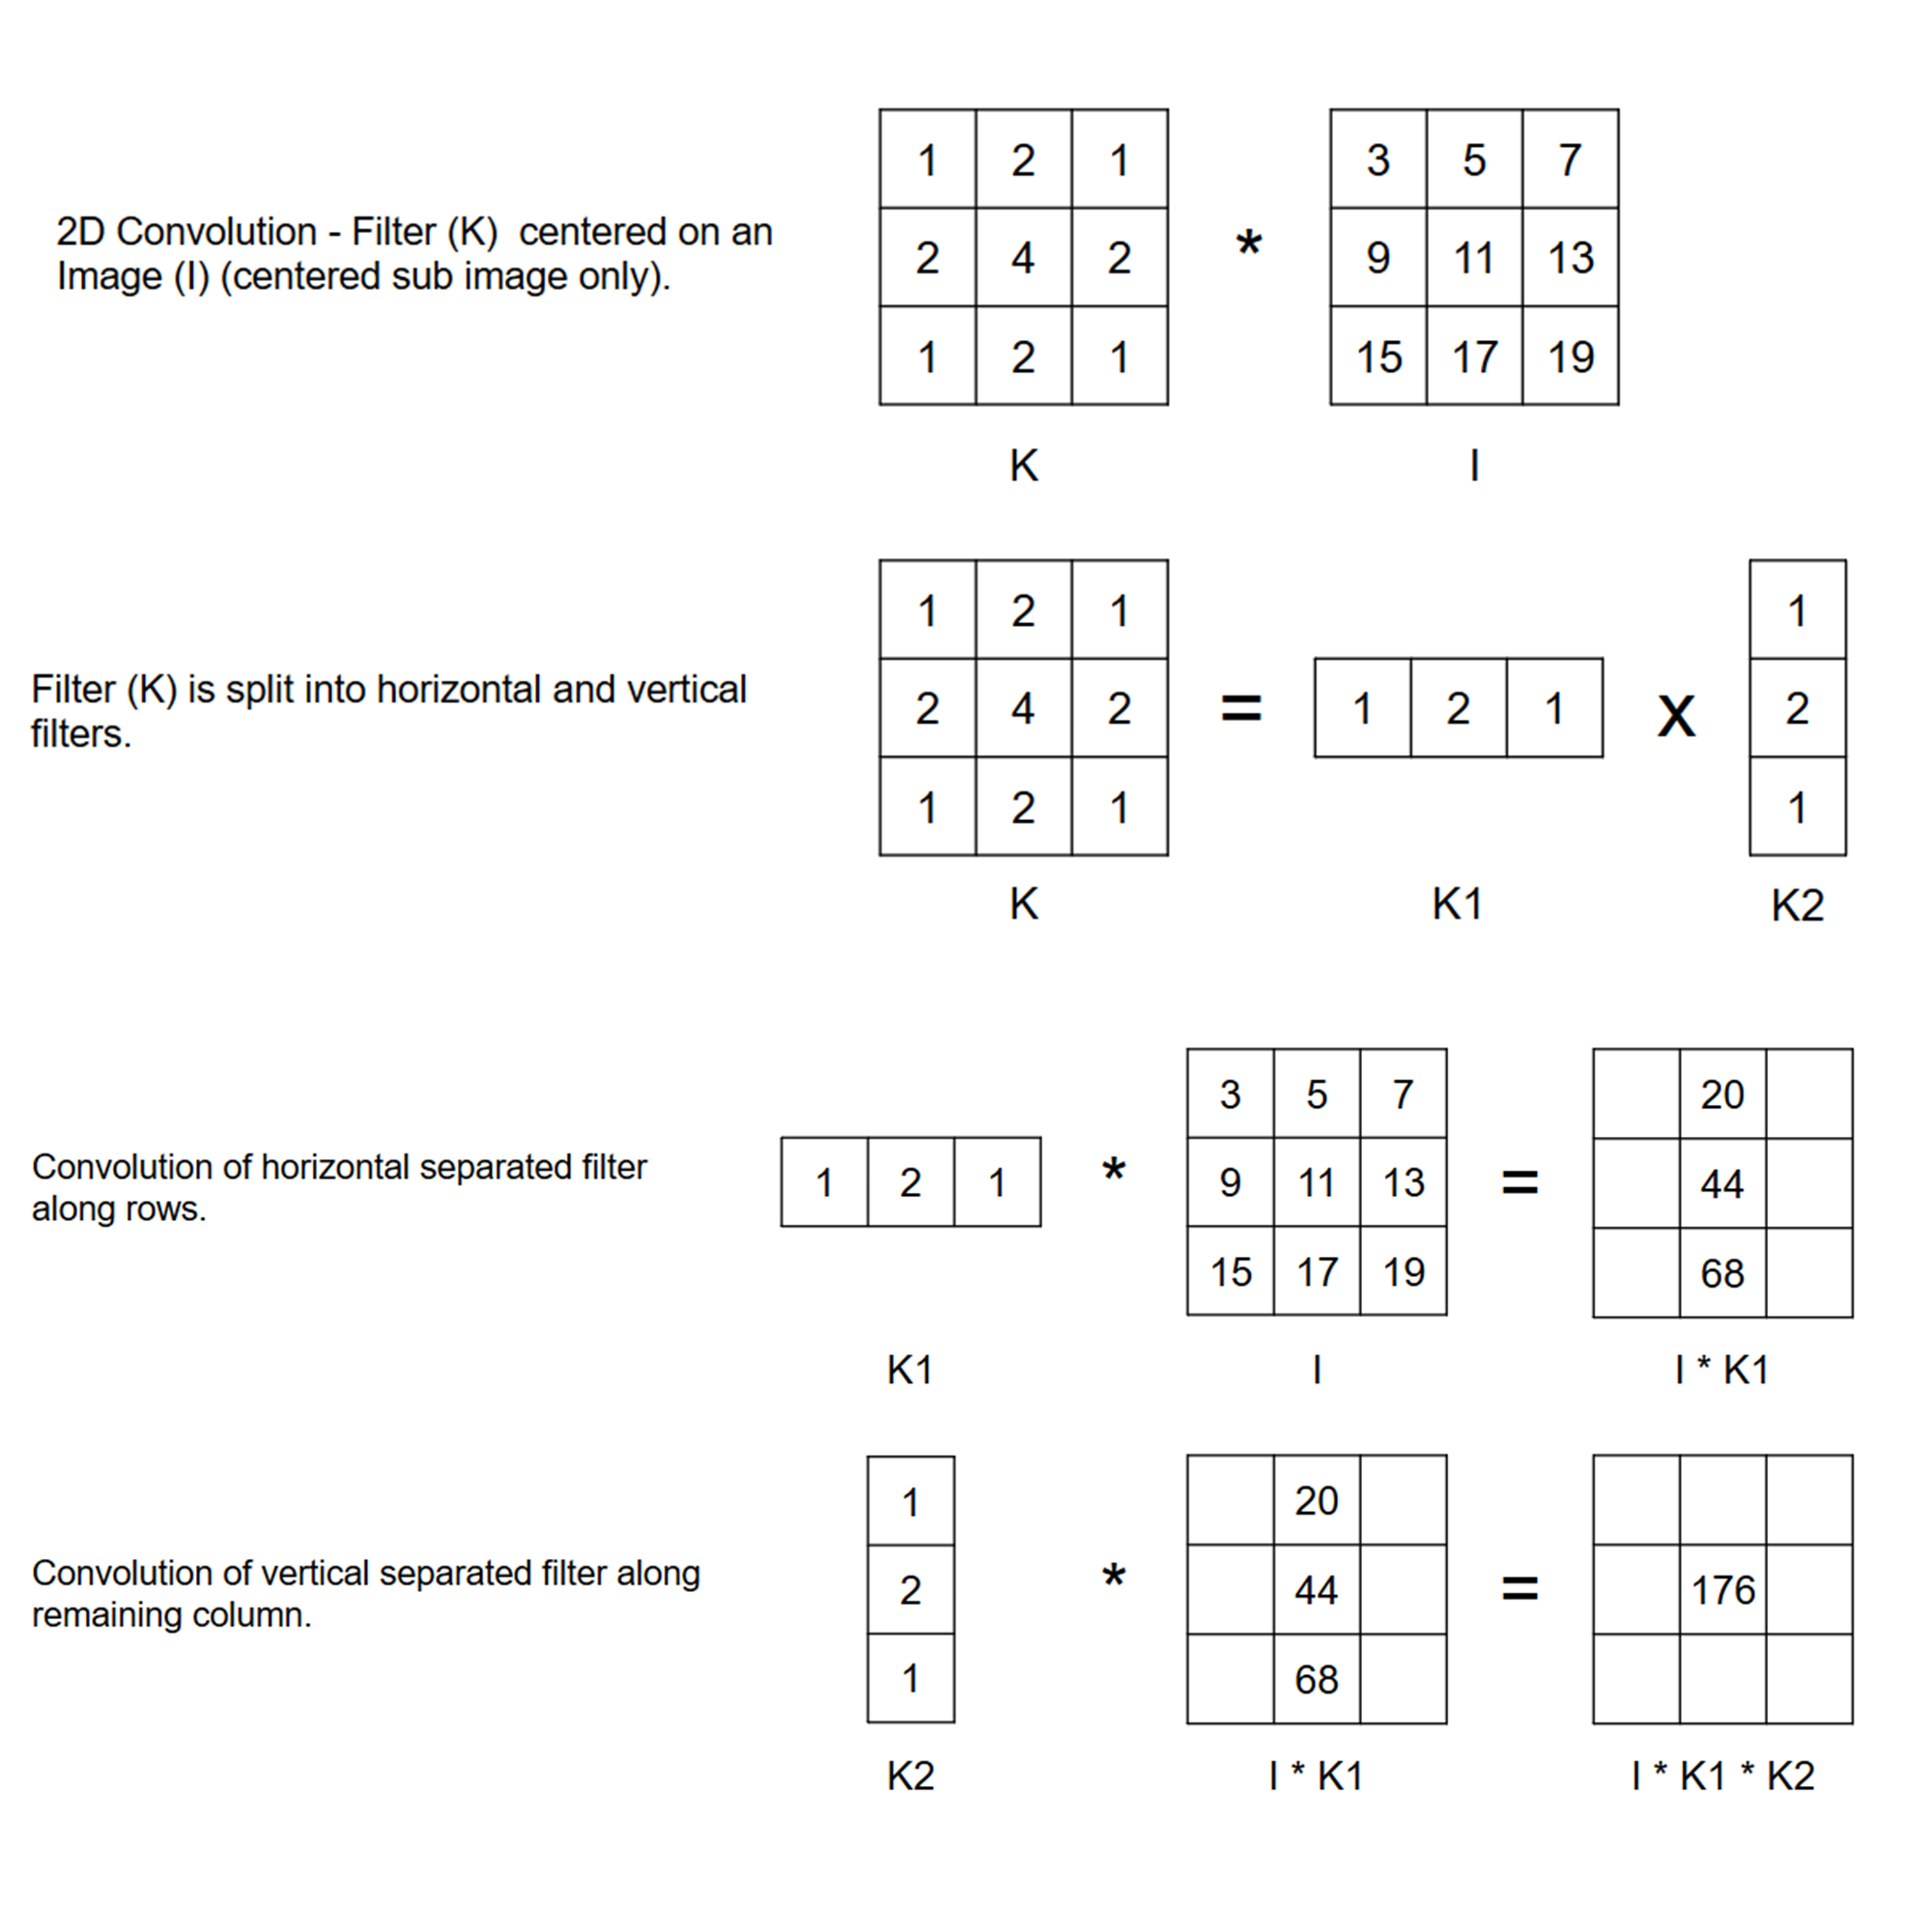
\includegraphics[width=0.7\linewidth]{images/separableconv}
\caption{Exemple d'un filtre de convolution appliqué successivement horizontalement puis verticalement}
\label{fig:conv:separable}
\end{figure}

Nous avons choisi de n'effectuer que l'optimisation sur carte graphique car la deuxième méthode comporte un gros coût en complexité et temps de développement que nous n'avons pas jugé nécessaire d'inclure dans cette première version. De plus, il n'est pas toujours possible de séparer un filtre $K$ en deux sous-filtres $K1, K2$ tel que $K = K1 \times K2$.

Pour pouvoir développer ladite optimisation, il a fallut utiliser un langage de programmation sur carte graphique. De nos jours, il en existe plusieurs et ils possèdent tous leurs spécificités. Cependant, pendant la phase de recherche, trois langages (ou sous-langages) se sont démarqués : OpenCL\cite{opencl}, OpenGL ES\cite{opengles} et CUDA\cite{cuda}. Par professionnalisme, nous avons choisi d'implémenter trois versions de l'algorithme de convolution naïf (non séparé) utilisant chacun de ces langages, et d'en évaluer les performances.

\subsection{OpenCL} 
OpenCL ou \emph{Open Computing Language} est un langage de programmation basé sur le C, créé par \texttt{Khronos Group} en 2009.
Un programme OpenCL s'écrit en deux parties : La partie \textbf{code hôte} et la partie \textbf{noyau} ou \textbf{code périphérique}, qui représentent respectivement la partie application se chargeant d'orchestrer les différentes tâches, la gestion mémoire ainsi que la gestion des périphériques s'exécutant sur l'hôte et la partie calcul permettant de compléter lesdites tâches s'exécutant sur les périphériques. La partie hôte est écrite en C tandis que la partie noyau est écrite en OpenCL-C.
Il faut donc aussi différencier hôte et périphérique (Figure~\ref{fig:opencl}). Dans notre cas d'utilisation, l'hôte représente le processeur et permet de transmettre les données aux périphériques qui, ici, correspondent à une ou plusieurs cartes graphiques.

\begin{figure}[H]
\centering
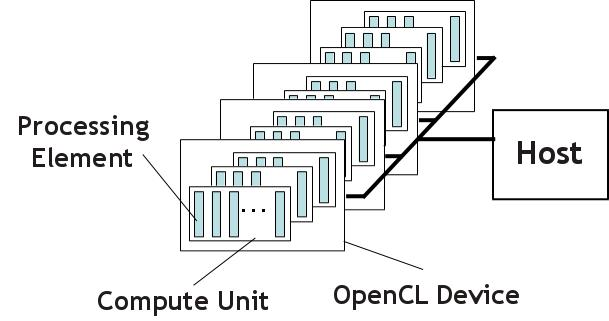
\includegraphics[width=0.5\linewidth]{images/opencl}
\caption{Schéma OpenCL - Hôte et périphériques\protect\footnotemark}
\label{fig:opencl}
\end{figure}

\footnotetext{Source: \href{https://www.anandtech.com/show/7334/a-look-at-alteras-opencl-sdk-for-fpgas/2}{https://www.anandtech.com/show/7334/a-look-at-alteras-opencl-sdk-for-fpgas/2}}

Nous nous sommes intéressés à OpenCL car il est compatible avec la plupart des systèmes et des architectures aujourd'hui présents sur le marché, sans aucune modification de code nécessaire. Cet avantage est aussi l'un de ses plus gros inconvénients puisqu'il ne permet pas d'exploiter au mieux chaque architecture comme peut le faire CUDA avec NVIDIA, et les performances de ce dernier ne sont donc pas équivalentes sur chaque architecture. %Parler dans le bilan Le coût de développement de traitement en OpenCL tout aussi lourd

\subsection{OpenGL (ES)}
OpenGL est une interface de programmation multi-plateforme et multi-langage permettant de faire le rendu de scènes 2D/3D. En tant qu'interface, il est possible de l'implémenter de façon logicielle mais elle a été conçue pour être implémentée de manière matérielle afin de profiter au mieux des accélérations matérielles disponibles. Ainsi, c'est grâce à ces implémentations qu'OpenGL fournit un \emph{pipeline} programmable de rendu ultra performant. C'est via ce pipeline programmable et plus spécifiquement via le code hôte et les shaders qu'il est possible de transmettre des instructions et des données à la carte graphique (Figure~\ref{fig:opengl:pipeline})

\begin{figure}[H]
\centering
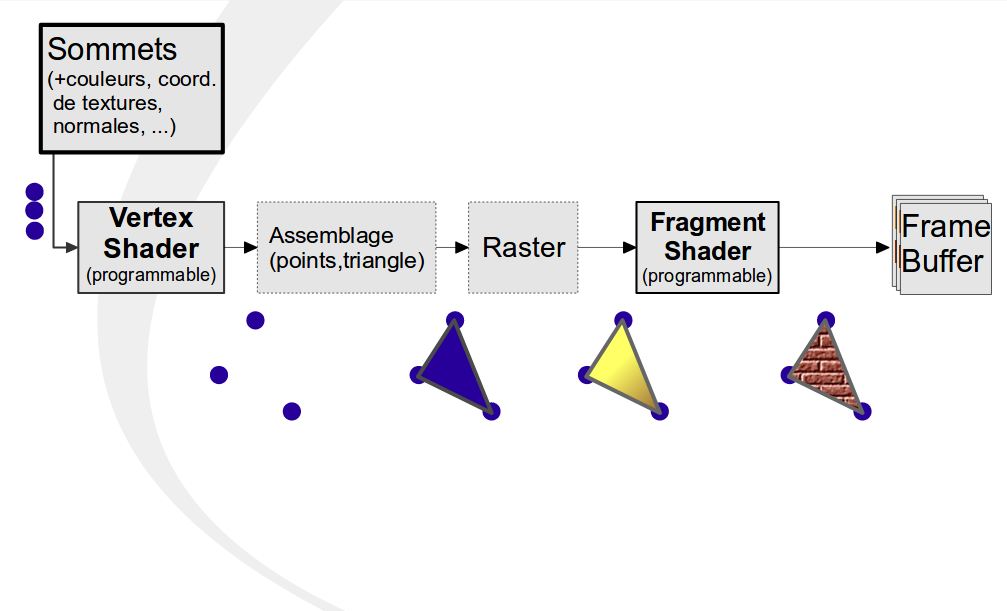
\includegraphics[width=0.7\linewidth]{images/opengl-pipeline}
\caption{Pipeline de rendu - OpenGL\protect\footnotemark}
\label{fig:opengl:pipeline}
\end{figure}

\footnotetext{Source: \href{http://www.labri.fr/perso/pbenard/teaching/mondes3d/slides/Cours_Monde3D_2017_04-IntroGL.pdf}{Cours M1 Informatique - Mondes 3D - Pierre Benard}}

Le pipeline OpenGL reçoit en entrée:
\begin{itemize}
\item Des informations sur la géométrie de la scène.
\item Des paramètres nécessaires pour effectuer le rendu de la scène (point de vue de la caméra, lumières, textures, matériaux).
\end{itemize}
et donne en sortie une image de la scène.

Pour pouvoir utiliser ce pipeline dans l'optique d'opérer des traitements sur des images 2D, il est nécessaire d'en détourner l'utilisation. En effet, sans géométrie à fournir au vertex shader, le pipeline de rendu ne se déclenche pas. L'idée, pour passer outre, est de créer un bout de géométrie recouvrant l'écran (le plus souvent un quad) afin d'activer le pipeline de rendu. Une fois activé, le vertex shader est programmé pour ne rien faire. Les étapes d'assemblage et de rastérisation sont, de ce fait, très rapidement achevées et l'étape du rendu par fragment peut alors débuter. L'image de sortie du rendu est composée dans le fragment shader, c'est donc ici que nous avons accès à chacun des pixels composant l'image finale. Le code présent dans ce shader permet d'effectuer, pour chaque pixel, le calcul de la convolution. Une fois le traitement par fragment effectué, l'image résultat est stockée dans le \emph{Frame Buffer Object ou FBO} et peut être récupérée depuis l'hôte.

L'avantage de cette technique est que, comme OpenCL, OpenGL (ES) est largement compatible avec toutes les plateformes et est très largement utilisé. Cependant, contrairement à OpenCL, les performances d'OpenGL ne dépendent que du matériel, ainsi, elles ne varieront pas, ou très peu, d'une architecture à un autre.

\subsection{CUDA} 
A la différence d'OpenCL et d'OpenGL, CUDA n'est pas seulement un langage de programmation mais bel et bien une architecture de traitement parallèle développée par NVIDIA. Son unique but est d'exploiter la carte graphique à son maximum, pour offrir une énorme puissance de calcul au système l'utilisant. Pour ce qui est de la partie programmation, NVIDIA fournit une API permettant d'utiliser cette architecture, CUDA C, et qui fonctionne de façon similaire à OpenCL avec du code hôte et du code périphérique qui seront les noyaux CUDA à exécuter sur la carte graphique. Là où CUDA se démarque c'est dans le modèle qu'il propose : les tâches (\emph{threads}) sont regroupées en blocs (\emph{blocks}) à l'intérieur desquels la mémoire est partagée. De plus, chaque bloc s'exécute sur exactement une unité de calcul (Figure~\ref{fig:cuda:archi}). Par ailleurs, la mémoire est unifiée (Figure~\ref{fig:cuda:unifiedmemory}), de ce fait, les CPUs et les GPUs travaillant ensemble ont accès à la même mémoire, ce qui permet d'éviter bon nombre de copies et ainsi réduire considérablement les temps de transfert de données.

\begin{figure}[H]
\centering
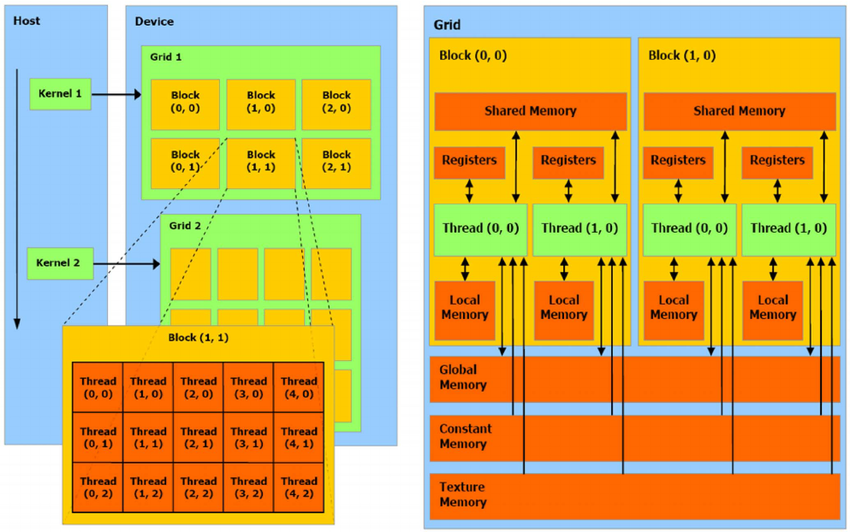
\includegraphics[width=0.9\linewidth]{images/cuda-archi}
\caption{Représentation schématique de l'architecture CUDA\protect\footnotemark}
\label{fig:cuda:archi}
\end{figure}
\footnotetext{Source: \href{http://programming4.us/enterprise/18672.aspx}{NVIDIA CUDA - Unified Device Architecture}}

\begin{figure}[H]
\centering
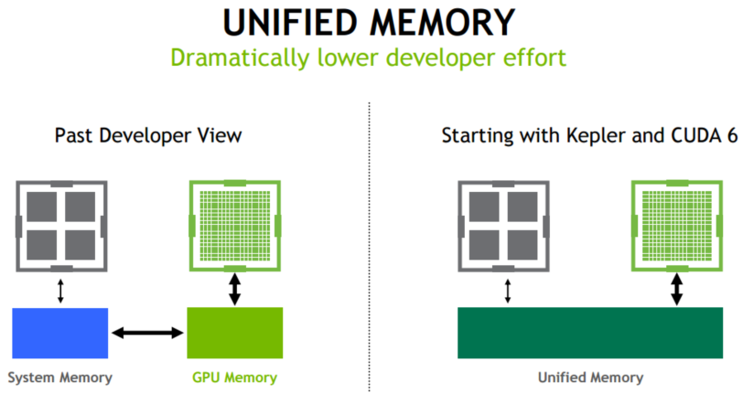
\includegraphics[width=0.65\linewidth]{images/cuda-unified-memory}
\caption{Mémoire séparée vs mémoire unifiée\protect\footnotemark}
\label{fig:cuda:unifiedmemory}
\end{figure}
\footnotetext{Source: \href{https://devblogs.nvidia.com/unified-memory-cuda-beginners/}{NVIDIA CUDA - Unified Memory for beginners}}

CUDA étant une architecture matérielle, seules les cartes graphiques NVIDIA récentes en sont équipées, ce qui, contrairement aux deux autres, ne la rend absolument pas multi-plateforme.

\subsection{Tests de performance}
\label{sub:conv:bench}
Afin de comparer les différentes solutions, nous avons réalisé des tests de performance du même algorithme de convolution, que nous avons implémenté dans les différents langages cités et sur différentes machines avec des configurations bien différentes. Le but de ces tests était, dans un premier temps, d'observer l'impact de l'optimisation et dans un second temps, d'orienter le choix d'ordinateur à inclure dans le système de RealityTech en se basant sur les résultats obtenus en fonction des différentes plateformes.

\textbf{Note:} L'algorithme de convolution implémenté est la version non séparé où le filtre de convolution est considéré comme une matrice.
\textbf{Note 2:} Nous avons choisit de ne pas réalisé les tests de performance OpenCL car nous avons jugé que cette technologie comportait beaucoup de trop de défauts et n'était donc pas pertinente.

Dans ce test de performance, nous avons mesuré plusieurs choses :
\begin{itemize}
\item \textbf{Le temps de transfert} des données de l'hôte au périphérique. Cette mesure est importante car elle permet d'évaluer l'impact de la mémoire unifiée CUDA par rapport aux autres méthodes ne possédant pas cette fonctionnalité.
\item \textbf{Le temps de calcul} brut de la convolution de l'image. Afin d'évaluer les performances brutes de l'algorithme par langage, nous avons mesuré les temps de calcul de chacun.
\item \textbf{La "bande passante"} du traitement entier, comprenant transfert calcul et re transfert. Cette mesure donne une bonne idée de la rapidité des algorithmes car elle exprime le nombre de méga octet qu'il est possible de traiter en une seconde avec chaque implémentation.
\end{itemize}

\textbf{Note:} Les résultats présentés dans les tableaux~\ref{fig:bench:cuda},~\ref{fig:bench:opengles},~\ref{fig:bench:cpu} ont été mesurés sur le kit de développement NVIDIA Tegra Jetson TX2 dont les spécificités sont les suivantes: \texttt{CPU ARM ARM Cortex-A57 (quad-core) @ 2GHz + NVIDIA Denver2 (dual-core) @ 2GHz, GPU 256-core Pascal @ 1300MHz, RAM 8GB 128-bit LPDDR4 @ 1866Mhz |  59.7 GB/s}. Nous avons choisi d'exposer ici seulement les résultats obtenus sur le kit de developpement NVIDIA car il permet d'observer les performances de CUDA dans un environnement ultra optimisé pour ce dernier cependant vous trouverez en Annexe 1 les résultats de ces mêmes tests effectués sur plusieurs ordinateurs différents.

\begin{table}[H]
\centering
\caption{CUDA 9.0 - Convolution d'une image en niveau de gris par un filtre de taille 5x5 - float 32bits}
\label{fig:bench:cuda}
\resizebox{\textwidth}{!}{%
\begin{tabular}{|c|c|c|c|c|c|}
\hline
\textbf{Size} & \textbf{Size (MB)} & \textbf{Compute Time (ms)} & \textbf{Transfer Time (ms)} & \textbf{Total Time (ms)} & \textbf{Bandwidth (MB/s)} \\ \hline
\cellcolor{green!40}\textbf{128x128} & 0,0655 & 0,0964 & 0,7737 & \cellcolor{green!40}0,8701 & 75,3224 \\ \hline
\cellcolor{green!40}\textbf{256x256} & 0,2621 & 0,2222 & 1,8457 & \cellcolor{green!40}2,0679 & 126,7661 \\ \hline
\cellcolor{green!40}\textbf{512x512} & 1,0486 & 0,8764 & 3,5266 & \cellcolor{green!40}4,4030 & 238,1503 \\ \hline
\cellcolor{green!40}\textbf{1024x1024} & 4,1943 & 3,2107 & 9,1959 & \cellcolor{green!40}12,4066 & 338,0703 \\ \hline
\cellcolor{orange!70}\textbf{2048x2048} & 16,7772 & 12,7048 & 35,0284 & \cellcolor{orange!70}47,7332 & 351,4786 \\ \hline
\cellcolor{red!40}\textbf{4096x4096} & 67,1089 & 51,0330 & 139,0710 & \cellcolor{red!40}190,1040 & 353,0115 \\ \hline
\cellcolor{red!40}\textbf{8192x8192} & 268,4350 & 210,2130 & 553,8050 & \cellcolor{red!40}764,0180 & 351,3464 \\ \hline
\end{tabular}%
}
\end{table}

\begin{table}[H]
\centering
\caption{OpenGL ES 2.0 - Convolution d'une image en niveau de gris par un filtre de taille 5x5 - float 32bits}
\label{fig:bench:opengles}
\resizebox{\textwidth}{!}{%
\begin{tabular}{|c|c|c|c|c|c|}
\hline
\textbf{Size} & \textbf{Size (MB)} & \textbf{Compute Time (ms)} & \textbf{Transfer Time (ms)} & \textbf{Total Time (ms)} & \textbf{Bandwidth (MB/s)} \\ \hline
\cellcolor{green!40}\textbf{128x128} & 0,0655 & 0,1386 & 0,9038 & \cellcolor{green!40}1,0424 & 62,8703 \\ \hline
\cellcolor{green!40}\textbf{256x256} & 0,2621 & 0,0202 & 1,3858 & \cellcolor{green!40}1,4060 & 186,4475 \\ \hline
\cellcolor{green!40}\textbf{512x512} & 1,0486 & 0,0194 & 4,2613 & \cellcolor{green!40}4,2807 & 244,9576 \\ \hline
\cellcolor{green!40}\textbf{1024x1024} & 4,1943 & 0,0212 & 15,6039 & \cellcolor{green!40}15,6251 & 268,4337 \\ \hline
\cellcolor{red!40}\textbf{2048x2048} & 16,7772 & 0,0215 & 60,8093 & \cellcolor{red!40}60,8309 & 275,8008 \\ \hline
\cellcolor{red!40}\textbf{4096x4096} & 67,1089 & 0,0215 & 241,5410 & \cellcolor{red!40}241,5625 & 277,8117 \\ \hline
\cellcolor{red!40}\textbf{8192x8192} & 268,4350 & 0,0267 & 1163,1867 & \cellcolor{red!40}1163,2133 & 230,7702 \\ \hline
\end{tabular}%
}
\end{table}

\begin{table}[H]
\centering
\caption{CPU - Convolution d'une image en niveau de gris par un filtre de taille 5x5 - float 32bits}
\label{fig:bench:cpu}
\resizebox{\textwidth}{!}{%
\begin{tabular}{|c|c|c|c|c|c|}
\hline
\textbf{Size} & \textbf{Size (MB)} & \textbf{Compute Time (ms)} & \textbf{Transfer Time (ms)} & \textbf{Total Time (ms)} & \textbf{Bandwidth (MB/s)} \\ \hline
\cellcolor{green!40}\textbf{128x128} & 0,0655 & 8,3513 & 0,0000 & \cellcolor{green!40}8,3569 & 7,8421 \\ \hline
\cellcolor{green!40}\textbf{256x256} & 0,2621 & 33,8604 & 0,0000 & \cellcolor{green!40}33,8698 & 7,7398 \\ \hline
\cellcolor{red!40}\textbf{512x512} & 1,0486 & 150,1860 & 0,0000 & \cellcolor{red!40}150,2010 & 6,9812 \\ \hline
\cellcolor{red!40}\textbf{1024x1024} & 4,1943 & 721,2130 & 0,0000 & \cellcolor{red!40}721,2310 & 5,8155 \\ \hline
\cellcolor{red!40}\textbf{2048x2048} & 16,7772 & 3196,6300 & 0,0000 & \cellcolor{red!40}3196,6500 & 5,2484 \\ \hline
\cellcolor{red!40}\textbf{4096x4096} & 67,1089 & 13130,9000 & 0,0000 & \cellcolor{red!40}13130,9000 & 5,1108 \\ \hline
\cellcolor{red!40}\textbf{8192x8192} & 268,4350 & 53591,6000 & 0,0000 & \cellcolor{red!40}53591,7000 & 5,0089 \\ \hline
\end{tabular}%
}
\end{table}

Comme on peut s'en rendre compte, les gains de performance des deux versions optimisées de l'algorithme sont non négligeables par rapport à la version CPU naïve (Figure~\ref{fig:bench:cpu}). En effet, on observe que les algorithmes s'exécutant sur la carte graphique sont jusqu'à 55 fois plus rapide pour OpenGL ES (Figure~\ref{fig:bench:opengles}) et jusqu'à 70 fois pour la version CUDA (Figure~\ref{fig:bench:cuda}). Les cases vertes dans les tableaux indiquent que l'image a pu être traitée en pseudo temps réel avec une fréquence de rafraichissement de 25fps, ce qui signifie que pour chaque image à afficher, nous disposons d'un temps de $1/25 * 1000 = 40$ millisecondes pour en faire le rendu. Au delà de ce constat d'optimisation, on peut voir que la version CUDA et la version OpenGL affichent des résultats plutôt similaires puisqu'ils sont tout deux capables de traiter en temps réel des images de taille 1024x1024 pixels sans difficulté. Toutefois, on note quand même une différence flagrante entre ces deux versions. En effet, on peut observer le gain apporté par la mémoire unifiée CUDA lorsque l'on compare les temps de transfert avec ceux d'OpenGL. En moyenne les temps de transfert en CUDA (pour des images haute résolution) sont environ deux fois plus rapide que leurs équivalents OpenGL ES, ce qui a un impact significatif sur les performances car ils correspondent à la majeure partie du temps d'exécution du programme.

\subsection{Conclusion}
Au vu des résultats obtenus section~\ref{sub:conv:bench} nous pouvons souligner deux choses :
\begin{itemize}
\item L'optimisation de l'algorithme utilisant un filtre de convolution séparé n'aura quasiment aucun impact sur les performances en OpenGL car les temps de calcul sont négligeables par rapport aux temps de transfert. Ainsi, seules les versions CUDA et CPU bénéficieront des améliorations qu'il peut potentiellement apporter.
\item CUDA et OpenGL fournissent tout deux des résultats semblables (avec une potentielle amélioration du côté CUDA) mais n'offrent pas les mêmes possibilités. Avec CUDA, l'algorithme ne peut tourner que sur des machines possédant une architecture compatible. Nous avons jugé que le gain apporté par rapport à OpenGL ES, qui lui est totalement compatible, n'était pas suffisant pour contrebalancer ce coût, c'est pourquoi nous avons choisi de continuer à utiliser et développer la version OpenGL ES.
\end{itemize}

\newpage
\section{Amélioration matérielle}
\label{sec:hardwareup}
Comme évoqué dans l'introduction, le deuxième axe d'amélioration de la technologie de \texttt{RealityTech} concerne l'aspect purement matériel du système qu'elle propose. Dans cette partie, nous avons essayé d'observer et de mesurer la "puissance" du matériel utilisé afin de déterminer les parties cruciales à améliorer.

En premier lieu, nous nous sommes intéressés à la latence des dispositifs d'acquisition. La latence est définie comme le temps écoulé entre l'acquisition et l'affichage d'une information. 
Nous nous sommes donc procurés de nombreuses caméras différentes dont nous avons mesuré les latences sur plusieurs ordinateurs. Certains ordinateurs possèdaient des capacités matérielles d'encodage vidéo (comme sur le NVIDIA Jetson TX2, obtenu pour l'occasion, et qui possède un module MSENC, un encodeur matériel\footnote{\href{https://www.nvidia.fr/autonomous-machines/embedded-systems-dev-kits-modules/}{NVIDIA Jetson TX2 - Charactéristiques des modules}}) ce qui nous a permis d'en évaluer l'impact sur la latence lors de l'obtention du flux vidéo. Mis à part le Jetson TX2 possédant une caméra embarquée, les mesures de la latence ont toutes été effectuées en utilisant GStreamer\cite{gstreamer} avec la même commande d'obtention du flux afin d'éviter au maximum les différences de mesure.

Pour mesurer la latence, nous avons utilisé la méthode dite "Glass to glass" qui est pratiquement la seule méthode employée actuellement. Pour effectuer une telle mesure il faut afficher sur un écran un chronomètre haute résolution, pointer la caméra sur l'écran, afficher le flux vidéo de la caméra, puis prendre une photo de l'écran avec le compteur et le flux vidéo de la caméra filmant ce compteur, côte a côte (Figure~\ref{fig:latency:glasstoglass}). La latence est finalement obtenue en faisant la soustraction des deux temps affichés par les compteurs. 

Cette méthode comporte certains défauts, le plus critique étant la résolution du chronomètre utilisé. En effet, la latence d'une caméra s'exprime en millisecondes, ainsi, pour avoir une mesure assez précise, le chronomètre doit avoir un taux de rafraichissement inférieur à la milliseconde, ce qui est extrêmement rare. Ensuite, le taux de rafraichissement et la latence de l'écran utilisé viennent également perturber les mesures. Dans notre cas, nous avons utilisé un chronomètre avec une résolution de l'ordre de 1 a 5 millisecondes\footnote{\href{https://stopwatch.onlineclock.net/}{Online stopwatch}} et un écran 120Hz avec 1 milliseconde de temps de latence ce qui devait réduire les imprécisions introduites dans nos mesures. Aussi, au lieu de prendre une photographie, nous avons décidé de réaliser des vidéos ralenties en 240 fps et d'afficher, en plus du chronomètre, une vidéo où 12 couleurs se succèdent à une fréquence 1Hz. Ainsi, en plus de la mesure du chronomètre, nous pouvons calculer grâce à la vidéo ralentie le nombre d'image qu'il faut pour qu'un changement de couleur dans la vidéo se reflète dans l'affichage du flux vidéo de la caméra. Étant donné que nous filmons à 240 fps, chaque image de la vidéo où le changement de couleur n'est pas reflété, correspond à $(1/240) * 1000 = 4,16$ millisecondes. Par exemple, si sur la vidéo ralentie, un changement de couleur met trois images à être reflété, alors la latence est de $3 x 4.16 = 12.48$ millisecondes à plus ou moins 4.16ms.

\begin{figure}[H]
\centering
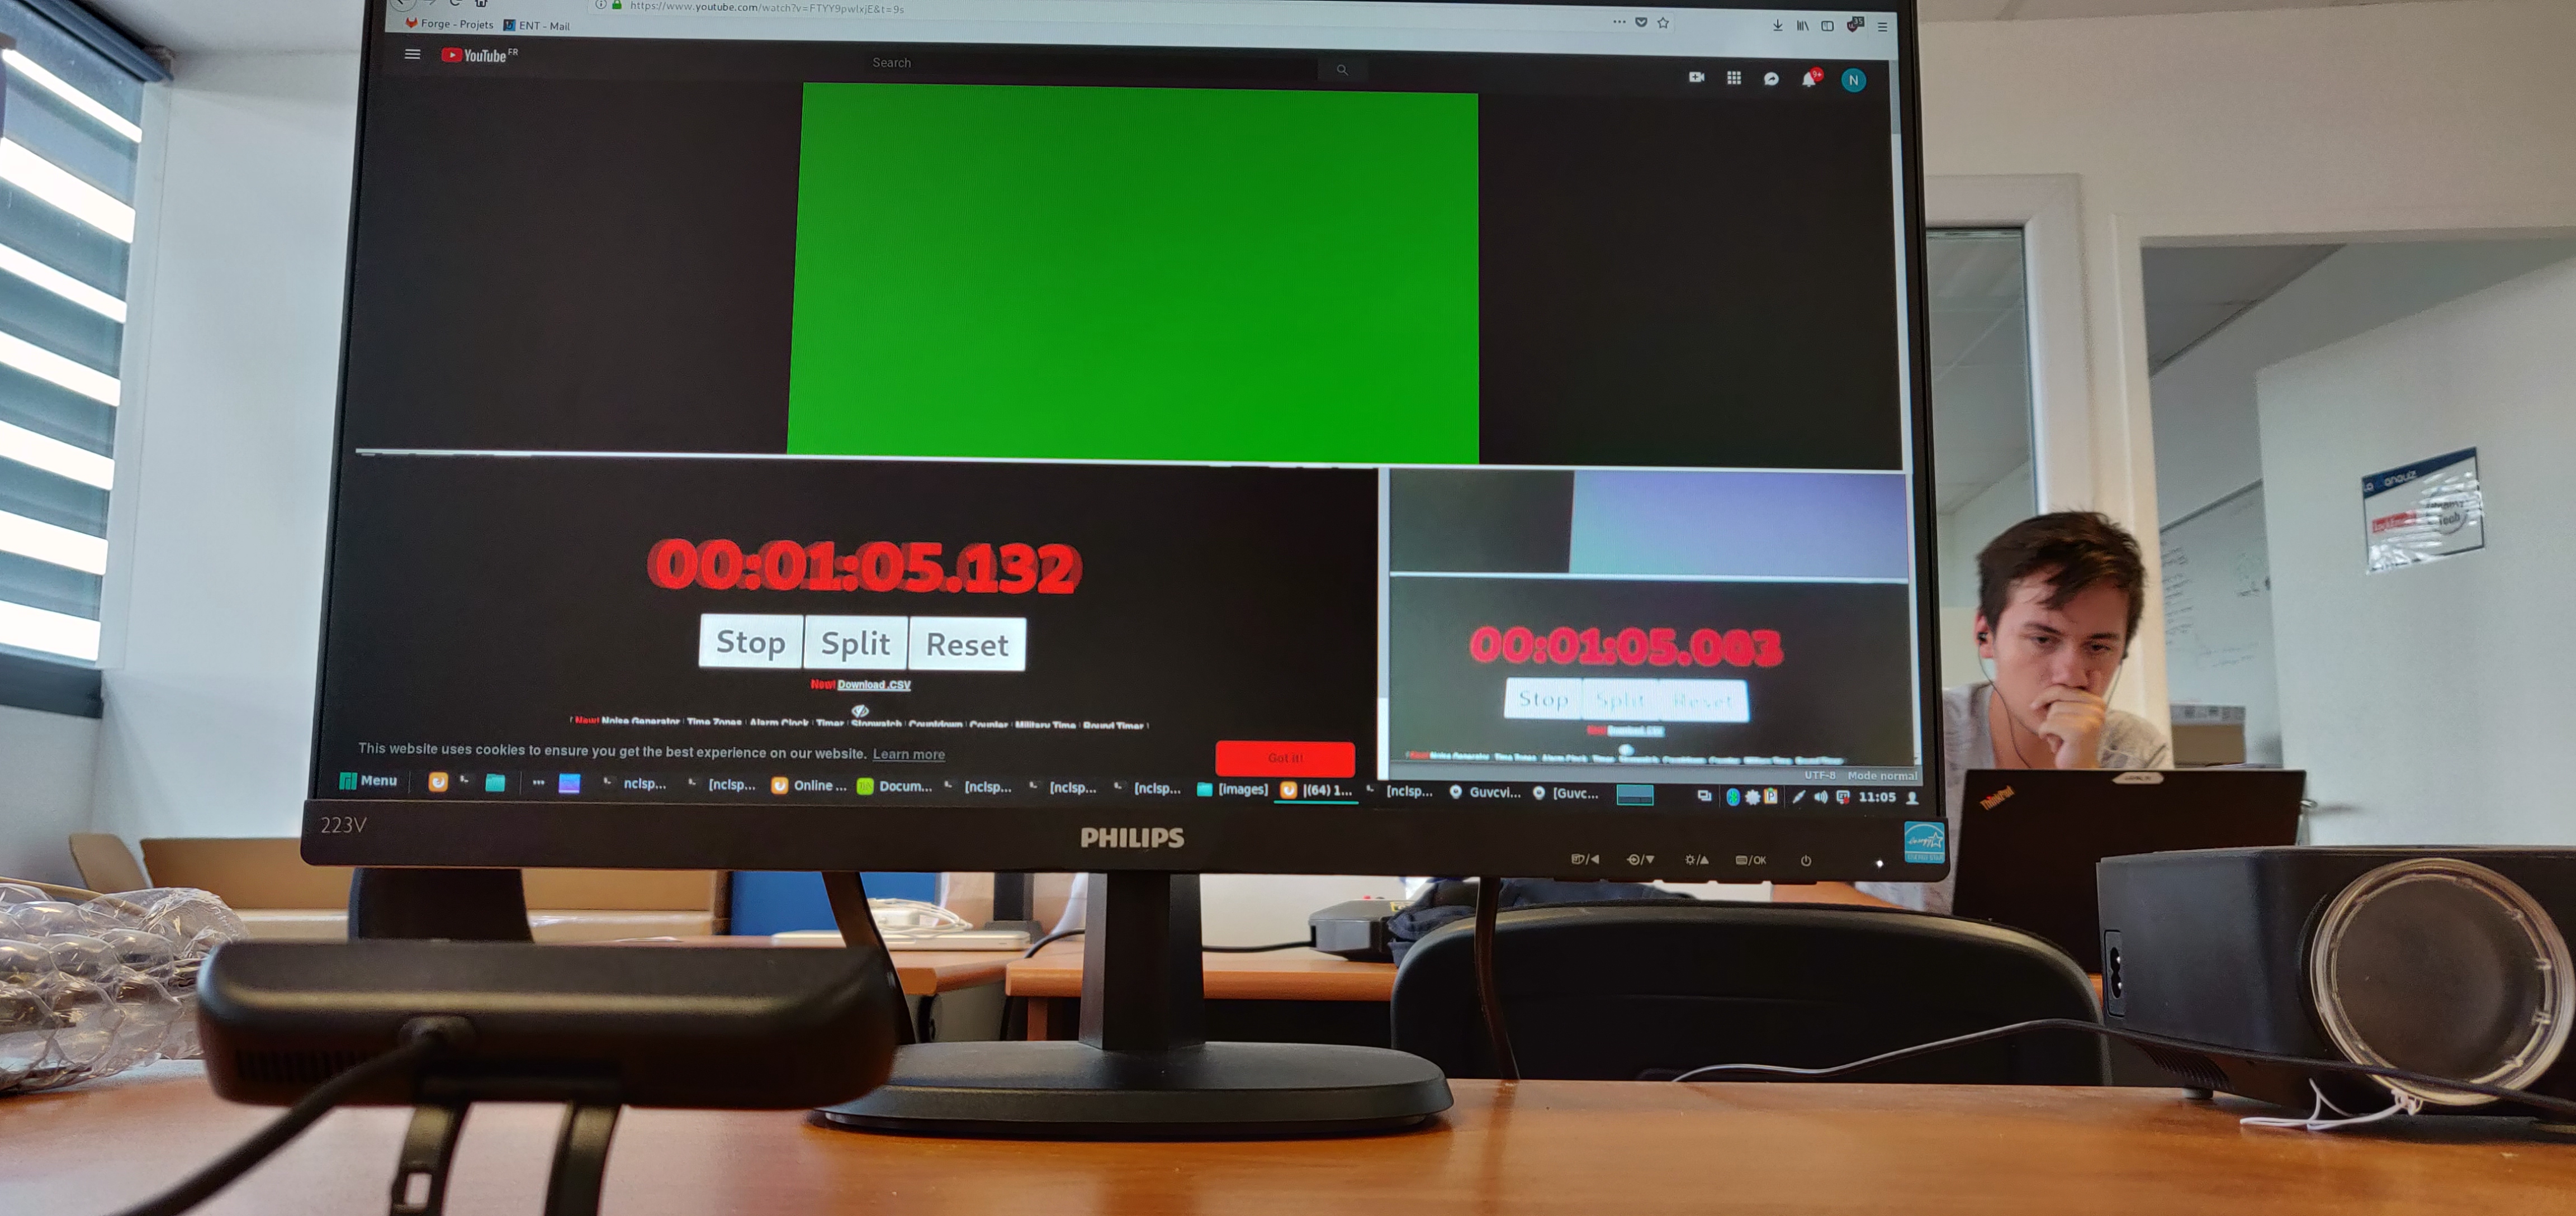
\includegraphics[width=\linewidth]{images/glasstoglass}
\caption{Exemple de mesure "glass to glass" de la latence d'une caméra}
\label{fig:latency:glasstoglass}
\end{figure}

Dans un soucis de cohérence avec la partie optimisation logicielle, vous trouverez dans le tableau~\ref{fig:latency:camera}, un comparatif des différentes latences de caméra obtenues sur le kit de développement NVIDIA Jetson TX2. Les résultats obtenus avec différents ordinateurs sont, quant à eux, présenter en Annexe 2.

\begin{table}[H]
\centering
\caption{Latence (en ms) de plusieurs caméras mesurée en Glass to glass - NVIDIA Jetson TX2}
\label{fig:latency:camera}
\resizebox{0.65\textwidth}{!}{%
\begin{tabular}{|c|c|c|c|c|c|c|}
\hline
\textbf{} & \textbf{Onboard (TX2)} & \textbf{Logitech} & \textbf{SR300} & \textbf{PSEye} & \textbf{Aukay} & \textbf{ELP} \\ \hline
\textbf{640x480} & 75 & 120 & \cellcolor{green!40} 70 & 120 & 85 & 80 \\ \hline
\textbf{1280x1020} & \cellcolor{green!40}80 & 80 & 85 & / & 85 & 85 \\ \hline
\textbf{1920x1080} & \cellcolor{green!40}80 & 130 & 300 & / & 170 & 95 \\ \hline 
\end{tabular}%
}
\end{table}

On s'aperçoit très rapidement que les tests de latence sont plutôt décevants. En effet, les latences sont toutes plus ou moins similaires même s'il y a quelques variations notamment pour la résolution 1920x1080, ce qui ne permet pas d'émettre beaucoup d'hypothèse d'amélioration. On observe que même la caméra embarquée (Onboard) disposant de son propre circuit intégré sur la carte mère du TX2 n'apporte aucun gain significatif par rapport aux autres caméras.
N'étant pas satisfait des résultats, nous avons décidé de mesurer la latence d'une caméra professionnelle \texttt{Point Gray} et la latence observée a été de seulement 8-10 millisecondes en résolution 1280x1020.

\newpage
\section{Nectar - Architecture micro services}
\label{sec:nectararchi}

Pour achever le développement du prototype haute performance, nous avons choisi de réétudier l'architecture logicielle de PapARt. 
Actuellement, PapARt est un gros kit de développement proposant une multitude de services regroupés en son sein comme par exemple l'acquisition du flux vidéo d'une caméra, le traitement des images, la détection de marqueurs, la visualisation, l'estimation de pose, etc.. Avec la centralisation des services, une panne peut être dramatique et rendre tout le système inutilisable. L'idée était donc de développer une nouvelle architecture pour pallier à ce défaut et permettre au système de gagner en réactivité, stabilité, performance, modularité et temps de maintenance. Une architecture en micro-services s'est imposée comme solution de choix car elle répond à tous les besoins énoncés.

Une architecture en microservices consiste à décomposer un logiciel en une multitude de services indépendants, effectuant chacun une tâche bien précise. Ces services peuvent ensuite communiquer les uns avec les autres par le biais d'une API.

\paragraph{Performance} Contrairement à une bibliothèque classique, avec une telle architecture il est possible d'allouer des ressources à la demande aux services en ayant besoin. Cela permet, par exemple, d'attribuer des ressources aux services les nécessitant lorsqu'un faible nombre d'entre eux est entrain de fonctionner. A la différence d'une bibliothèque classique où les ressources supplémentaires allouées l'auraient été pour tous les services. Ce gain de performance n'est pas négligeable car il permet d'améliorer considérablement la gestion des ressources, qui peut devenir critique en cas de saturation notamment.

\paragraph{Réactivité} Dans le cas d'une panne d'un service critique, tel que le service récupérant le flux vidéo de la caméra, avec une architecture centralisée la gestion de cette panne est très complexe et nécessite souvent de redémarrer tout le système, ce qui prend un certain temps. En revanche, une architecture en microservices couplée à un gestionnaire de processus se chargera uniquement de relancer le service en panne et, s'il le faut, les services associés, de manière quasiment transparente pour l'utilisateur.

\paragraph{Modularité} L'architecture en microservices offre une très grande modularité ; chaque service peut être écrit dans n'importe quel langage et peut être intégré au système sans coût tant qu'il respecte l'API de communication inter processus s'il n'est pas totalement indépendant. Il est ainsi très facile pour n'importe qui de rajouter des modules venant soit compléter un service existant soit tout simplement rajouter une fonctionnalité au système. Par exemple, un service d'estimation de pose peut être complété par un service de filtrage de façon totalement transparente à l'utilisateur final. L'utilisation ou non du filtrage peut être contrôlée de façon automatique par un autre module gérant par exemple la qualité générale voulue par l'utilisateur.

\paragraph{Maintenabilité} Lorsqu'un service est défectueux, le problème peut être très rapidement identifié car les services sont très faiblement couplés et ainsi il n'est souvent pas nécessaire de devoir parcourir une grande quantité de code pour pouvoir identifier un bug. De plus, grâce à la modularité de l'architecture, un service en maintenance n'affecte pas la stabilité générale du système.

\begin{figure}[H]
\centering
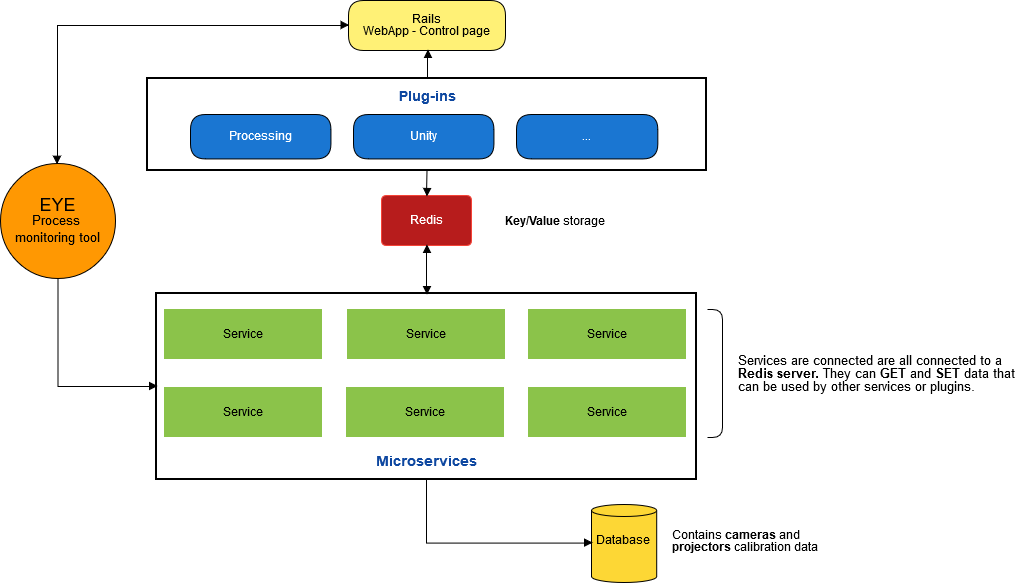
\includegraphics[width=\linewidth]{images/archi3}
\caption{Schéma de l'architecture en microservices développée}
\label{fig:microarchi}
\end{figure} 

Pour mettre en place cette nouvelle architecture (Figure~\ref{fig:microarchi}), nous nous sommes basés sur trois technologies principales :
\begin{itemize}
\item \textbf{Redis}\cite{redis} ou \emph{REmote DIctionnary Server} est un système de stockage clef-valeur qui, contrairement aux bases de données plus conventionnelles, stocke les données directement dans la mémoire vive (RAM) de l'ordinateur ou dans la mémoire virtuelle\footnotetext{\href{https://fr.wikipedia.org/wiki/Mémoire_virtuelle}{Wikipédia - Mémoire virtuelle}} et non pas sur le disque. Cette spécificité permet à Redis d'atteindre des performances inégalées par des bases de données classiques et il s'impose donc comme un choix de qualité pour nos besoins.
\item \textbf{Eye}\cite{eye} est un outil de gestion de processus qui permet de s'assurer du cycle de vie des processus qu'il gère. Eye offre la possibilité de lancer/redémarrer/couper automatiquement des processus en fonction de leur état, de leur dépendance et de leur consommation en ressource (mémoire, CPU). Il est ainsi possible de définir, pour chaque service, de quoi il dépend et quelles sont les ressources maximales qui lui sont autorisées, ce qui permet d'éviter la mise en péril de tout le système lorsqu'un processus commence à consommer 99\% de la mémoire disponible par exemple.
\item \textbf{Ruby on Rails}\cite{rubyrails} est un \emph{framework} destiné à la création d'applications web modernes rapidement et simplement. L'idée est d'utiliser Rails pour générer une page web de contrôle du système permettant de lancer/couper des processus, effectuer des tests et tout autre action permettant d'observer l'état général du système.
\end{itemize}

Dans notre architecture, tous les microservices sont connectés à Redis. Ils peuvent chacun manipuler les données présentes et en écrire de nouvelles. C'est uniquement par ce biais que se fait la communication inter services. Ainsi, par exemple, un service accédant à la caméra ne transfère pas directement ses données à un service analysant l'image, mais envoie l'image courante de la caméra dans Redis qui est ensuite récupérée par cet autre service. En outre, Redis possède une pipeline événementiel. Ce pipeline permet aux clients Redis (services) écoutant ou publiant sur une clé de notifier ou d'être notifié d'autres / par d'autres services. De ce fait, dès que des nouvelles données seront publiées sur une clé écoutée par des clients, ceux-ci recevront instantanément lesdites données. C'est ce pipeline que nous avons choisi d'utiliser pour éviter l'attente active des services et ainsi améliorer les performances générales du système.

Couplé à Redis, c'est Eye qui s'assure à tout moment que tous les services demandés par l'utilisateur sont en train d'être exécutés. Pour cela, il vérifie que le service est en marche mais aussi que toutes les dépendances sont satisfaites. Eye peut recevoir des commandes de l'application web qui est elle-même manipulée, soit par l'utilisateur soit par un module de développement. Les modules de développement sont des API permettant aux utilisateurs développeurs de créer leurs propres applications de réalité augmentée spatiale utilisant le système de RealityTech.

\section{Bilan}
Après avoir réalisé puis testé indépendamment chacune des parties composant le prototype haute performance, la dernière étape consistait à tester ce dernier, de bout en bout, dans un cas d'utilisation réelle. Le but de cet ultime test étant d'évaluer si le prototype remplit, ou non, les objectifs que nous nous sommes fixés à savoir : performance, réactivité, modularité et maintenabilité. 
Pour effectuer ce test, il fallait développer une application utilisant ce prototype. Pour ce faire, nous avions besoin du module Unity le mettant à profit. Le développement du module Unity ainsi que de l'application est détaillé section blabla.
A ce jour, le module et l'application n'étant toujours pas terminés, le test n'a pas encore été réalisé.